% Build this with LuaLaTeX or see below.

% Mandatory if you want to build in LuaLaTeX with the `standalone`class
% just remove it to build with another engine.
\RequirePackage{luatex85}
\documentclass[crop,tikz]{standalone}  % You can obviously change this to any class you want
% The following four lines are required, since we use those libraries
\usepackage{tikz}
    \usetikzlibrary{positioning}
    \usetikzlibrary{calc}
    \usetikzlibrary{shapes.multipart}

\begin{document}
% You can put your own tikzpicture instead of this one, which is the one `ginger` generates from `example.conll`
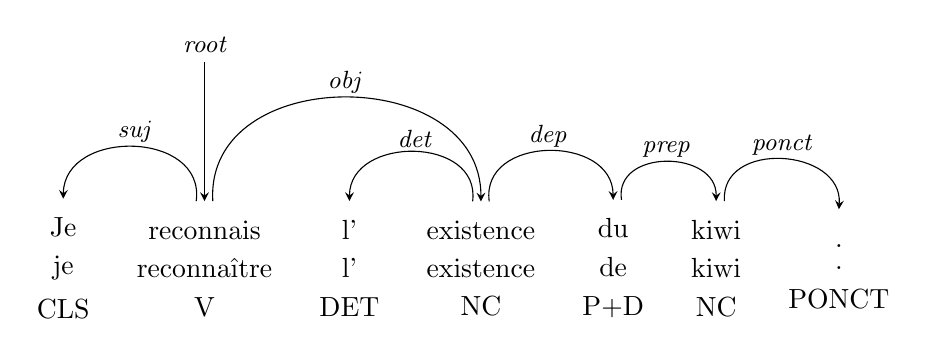
\begin{tikzpicture}[>=stealth, token/.style={text height=1em, rectangle split, rectangle split parts=3},
                               dep/.style={font=\small\itshape, midway, above=-.2em},
                               root/.style={font=\small\itshape, above}]
    \path[anchor=base]
        node[token] (t1) {Je\nodepart{two}je\nodepart{three}CLS}
        node[token, right=1em of t1] (t2) {reconnais\nodepart{two}reconnaître\nodepart{three}V}
        node[token, right=1em of t2] (t3) {l'\nodepart{two}l'\nodepart{three}DET}
        node[token, right=1em of t3] (t4) {existence\nodepart{two}existence\nodepart{three}NC}
        node[token, right=1em of t4] (t5) {du\nodepart{two}de\nodepart{three}P+D}
        node[token, right=1em of t5] (t6) {kiwi\nodepart{two}kiwi\nodepart{three}NC}
        node[token, right=1em of t6] (t7) {.\nodepart{two}.\nodepart{three}PONCT};
    \begin{scope}[local bounding box=arcs]
        \draw[->] ($(t2.north)+(-.3em, 0)$) .. controls ($(t2.north)!0.5!-90:(t1.north)$) and ($(t1.north)!0.5!-270:(t2.north)$) .. (t1.north) node[dep] {suj};
        \draw[->] ($(t4.north)+(-.3em, 0)$) .. controls ($(t4.north)!0.5!-90:(t3.north)$) and ($(t3.north)!0.5!-270:(t4.north)$) .. (t3.north) node[dep] {det};
        \draw[->] ($(t2.north)+(.3em, 0)$) .. controls ($(t2.north)!0.5!90:(t4.north)$) and ($(t4.north)!0.5!270:(t2.north)$) .. (t4.north) node[dep] {obj};
        \draw[->] ($(t4.north)+(.3em, 0)$) .. controls ($(t4.north)!0.5!90:(t5.north)$) and ($(t5.north)!0.5!270:(t4.north)$) .. (t5.north) node[dep] {dep};
        \draw[->] ($(t5.north)+(.3em, 0)$) .. controls ($(t5.north)!0.5!90:(t6.north)$) and ($(t6.north)!0.5!270:(t5.north)$) .. (t6.north) node[dep] {prep};
        \draw[->] ($(t6.north)+(.3em, 0)$) .. controls ($(t6.north)!0.5!90:(t7.north)$) and ($(t7.north)!0.5!270:(t6.north)$) .. (t7.north) node[dep] {ponct};
    \end{scope}

    \draw[->] ($(arcs.north west)!(t2.north)!(arcs.north east)$) node[root] {root} -- (t2.north);
\end{tikzpicture}
\end{document}
